\documentclass{beamer}
\usetheme[progressbar=frametitle]{metropolis}           % Use metropolis theme
\setbeamertemplate{frame numbering}[fraction]
\metroset{background=dark} % change background theme according to manual

% packages for pgf figure
\usepackage{tikz}
\usepackage{pgfplots}

\usepackage{hyperref}
\usepackage{graphicx} % package to use links

\setbeamercolor{palette primary}{bg=black,fg=white}
\setbeamercolor{background canvas}{parent=palette primary}
\setbeamercolor{normal text}{fg=white}
\setbeamercolor{progress bar}{use=palette primary,fg=red}

\setbeamersize{text margin left=1em,text margin right=1em}

%\usecolortheme{crane}

\title{Presentation}
\subtitle{Subtitle}
\date{\today}
\author{Federico Tartarini}
\institute{BEARS - Theme A}

\begin{document}
    \maketitle

    \begin{frame}{Latex - Brief introduction}
        \LaTeX is a high-quality typesetting system.
        \begin{itemize}
            \item it includes features designed for the production of technical and scientific documentation.
            \item \LaTeX is the de facto standard for the communication and publication of scientific documents.
            \item \LaTeX is available as free software.
        \end{itemize}
    \end{frame}

    \begin{frame}{Results}
        \centering
        \begin{figure}[]
            \centering
            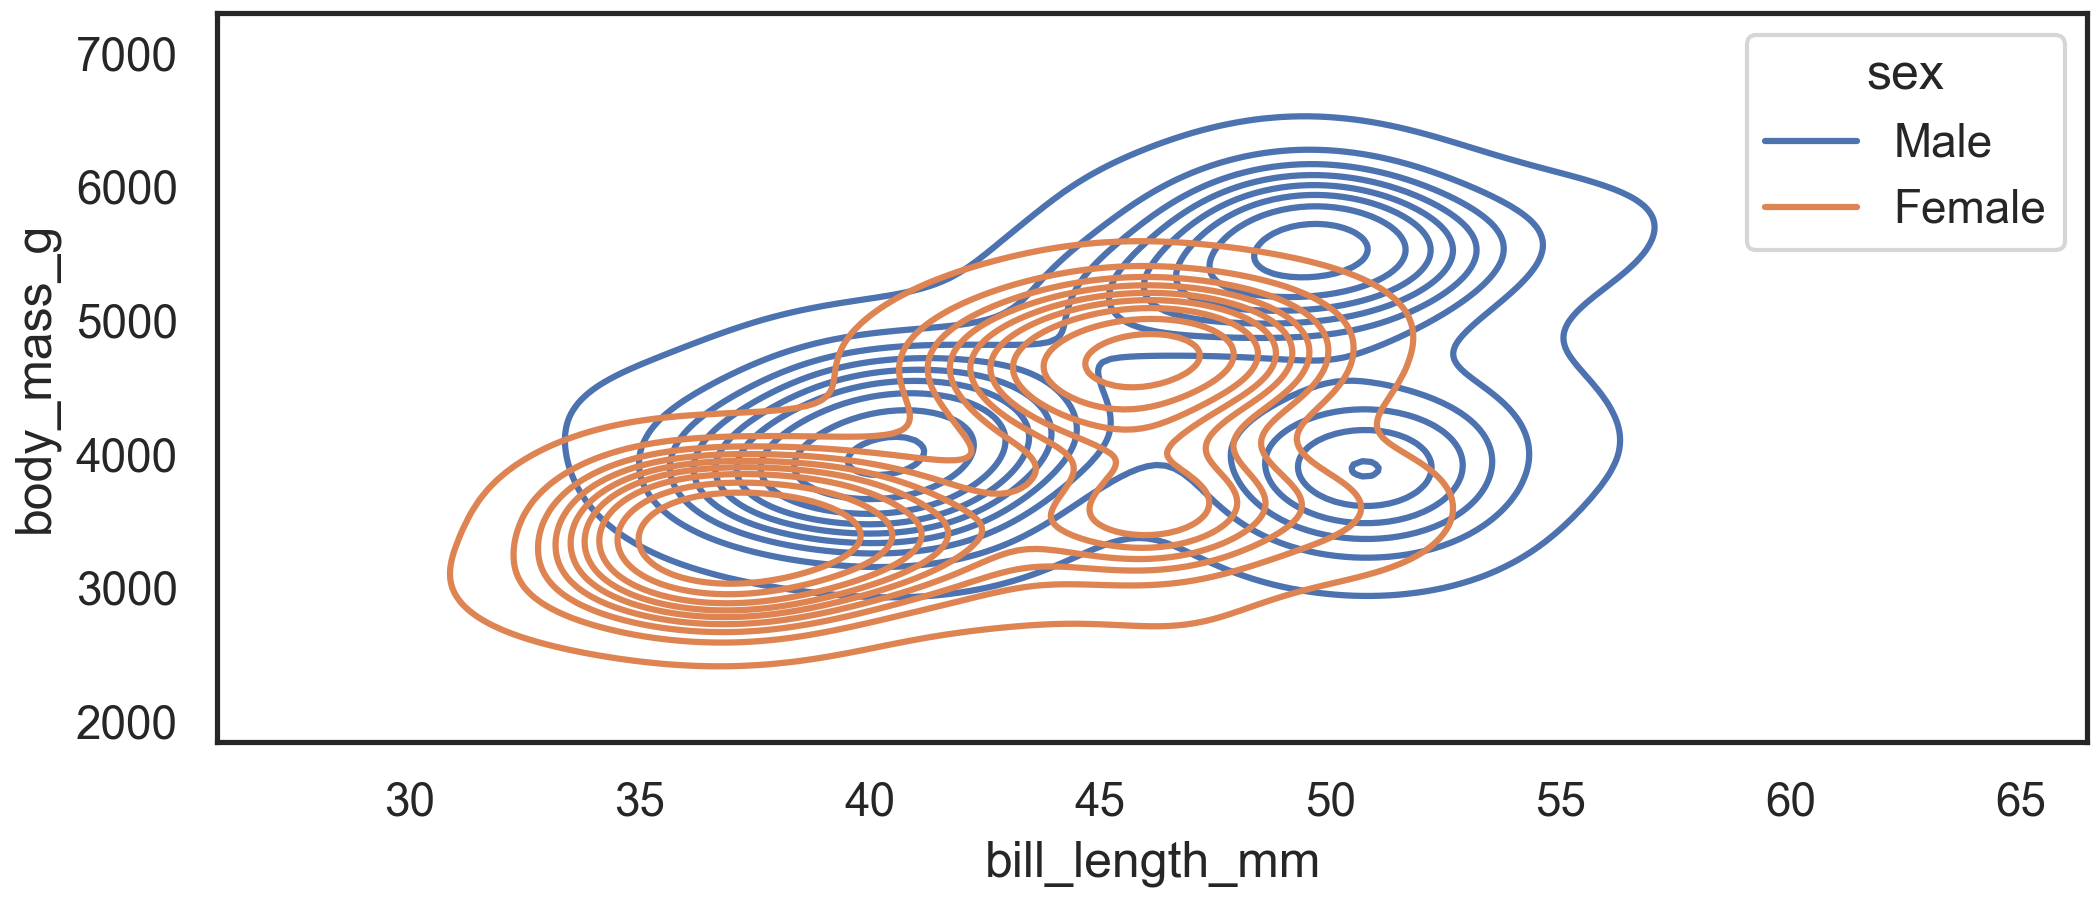
\includegraphics[width=\linewidth]{figures/penguins_distribution.png}
            \caption{Penguins.}
            \label{fig:penguins}
        \end{figure}
    \end{frame}

    \begin{frame}{Results}
        \begin{columns}
            \begin{column}{0.5\textwidth}
                \begin{enumerate}
                    \item Sample size 20 participants
                    \item Duration 180 days
                    \item Minimum of 42 surveys per week
                \end{enumerate}
            \end{column}
            \begin{column}{0.5\textwidth}
                \begin{enumerate}
                    \item Sample size 20 participants
                    \item Duration 180 days
                    \item Minimum of 42 surveys per week
                \end{enumerate}
            \end{column}
        \end{columns}
    \end{frame}
\end{document}